%File: formatting-instruction.tex
\documentclass[letterpaper]{article}
\usepackage{aaai}
\usepackage{times}
\usepackage{helvet}
\usepackage{courier}
\usepackage{graphicx}
\usepackage{amssymb}
\usepackage{amsmath}
\usepackage{amssymb}
\usepackage{color}
\usepackage{tikz}
\usepackage{pgfplots}
\usepackage{caption}
\usepackage{subcaption}
\usepackage{comment}
\usepackage{booktabs}
\usepackage{nopageno}
\usepackage{url}
\usepackage{chessboard}
\usepackage{skak}
\usepackage{amsthm}
\usepackage{amssymb}
\usepackage{amsmath}


\usepackage[algo2e, noend, noline, linesnumbered]{algorithm2e}
\providecommand{\SetAlgoLined}{\SetLine}  
\providecommand{\DontPrintSemicolon}{\dontprintsemicolon}
\DontPrintSemicolon
\makeatletter
\newcommand{\pushline}{\Indp}% Indent
\newcommand{\popline}{\Indm}
\makeatother
\newcommand{\argmax}{\operatornamewithlimits{argmax}}
\newcommand{\defword}[1]{\textbf{\boldmath{#1}}}

\captionsetup{compatibility=false}

%\pgfplotsset{compat=newest}
\usetikzlibrary{arrows,shapes,petri}

\newcommand{\bE}{\mathbb{E}}
\newcommand{\bQ}{\bar{Q}}
\newcommand{\cA}{\mathcal{A}}
\newcommand{\cC}{\mathcal{C}}
\newcommand{\cD}{\mathcal{D}}
\newcommand{\cG}{\mathcal{G}}
\newcommand{\cI}{\mathcal{I}}
\newcommand{\cN}{\mathcal{N}}
\newcommand{\cO}{\mathcal{O}}
\newcommand{\cR}{\mathcal{R}}
\newcommand{\cS}{\mathcal{S}}
\newcommand{\cT}{\mathcal{T}}
\newcommand{\cZ}{\mathcal{Z}}
\newcommand{\hQ}{\hat{Q}}
\newcommand{\hV}{\hat{V}}
\newcommand{\eg}{{\it e.g.,}~}
\newcommand{\ie}{{\it i.e.,}~}
\newtheorem{definition}{Definition}
\newtheorem{fact}{Fact}
\newtheorem{theorem}{Theorem}
\newtheorem{corollary}{Corollary}
\newtheorem{lemma}{Lemma}
\newtheorem{proposition}{Proposition}
\newcommand{\Proof}{{\noindent\bf Proof. }}
\newcommand{\citejustyear}[1]{\cite{#1}}
\newcommand{\Qed}{$\blacksquare$}
\newcommand{\abs}[1]{\left|#1\right|}
\newcommand{\todo}[1]{{\color{red}{\bf #1}}}
\newcommand{\breturn}{{\bf return}\xspace}

% the note center!
\definecolor{darkgreen}{RGB}{0,125,0}
\newcounter{nsNoteCounter}
\newcounter{mlNoteCounter}
\newcounter{mwNoteCounter}
\newcounter{tpNoteCounter}
\newcommand{\nsnote}[1]{{\scriptsize \color{blue} $\blacksquare$ \refstepcounter{vlNoteCounter}\textsf{[NS]$_{\arabic{vlNoteCounter}}$:{#1}}}}
\newcommand{\mlnote}[1]{{\scriptsize \color{darkgreen} $\blacksquare$ \refstepcounter{mlNoteCounter}\textsf{[ML]$_{\arabic{mlNoteCounter}}$:{#1}}}}
\newcommand{\mwnote}[1]{{\scriptsize \color{red} $\blacktriangle$ \refstepcounter{asNoteCounter}\textsf{[AS]$_{\arabic{asNoteCounter}}$:{#1}}}}
\newcommand{\tpnote}[1]{{\scriptsize \color{orange} $\blacktriangle$ \refstepcounter{asNoteCounter}\textsf{[TP]$_{\arabic{asNoteCounter}}$:{#1}}}}
%\newcounter{NoteCounter}
%\newcommand{\vlnote}[1]{{\scriptsize \color{blue} \refstepcounter{vlNoteCounter}\textsf{[VL]$_{\arabic{vlNoteCounter}}$:{#1}}}}
%\renewcommand{\vlnote}[1]{}


\frenchspacing
\setlength{\pdfpagewidth}{8.5in}
\setlength{\pdfpageheight}{11in}
\pdfinfo{
/Title (Insert Your Title Here)
/Author (Put All Your Authors Here, Separated by Commas)}
\setcounter{secnumdepth}{0}  

\begin{document}
% The file aaai.sty is the style file for AAAI Press 
% proceedings, working notes, and technical reports.
%
\title{Monte Carlo Tree Search with Heuristic Evaluations\\using Implicit Minimax Backups}
\author{Authors}

\maketitle

\begin{abstract}
Monte Carlo Tree Search (MCTS) has improved the performance of game-playing engines in 
domains such as Go, Hex, and general-game playing. MCTS has been shown to outperform
outperform classic alpha-beta search in games where good heuristic evaluations are difficult to obtain. 
In recent years, combining ideas from traditional minimax search in MCTS has been shown to be advantageous in some domains, 
such as Lines of Action, Amazons, and Breakthrough.
In this paper, we propose 
a new way to use heuristic evaluations to guide the MCTS search by storing the two sources of 
information, estimated win rates and heuristic evaluations, separately. 
Rather than using the heuristic evaluations to replace the playouts, 
our technique backs them up {\it implicitly} during its MCTS simulations. 
These learned evaluation values are then used to guide future simulations. 
Compared to current techniques, we show that using implicit minimax backups  
leads to stronger play performance in Breakthrough, Lines of Action, and Kalah. 
\end{abstract}

%\subsection{Related Work}

\section{Introduction}

Monte Carlo Tree Search (MCTS)~\cite{Coulom06Efficient,Kocsis06Bandit} is a simulation-based best-first
search paradigm that has been shown to increase performance in domains such as turn-taking games, 
general-game playing, real-time strategy games, single-agent planning, and more~\cite{mctssurvey}. 
While the initial applications have been to games where heuristic evaluations are difficult to obtain, 
progress in MCTS research has shown that heuristics can be effectively be combined in MCTS, even in games 
where classic minimax search has traditionally been preferred. 

The most popular MCTS algorithm is UCT~\cite{Kocsis06Bandit}, 
which performs a single simulation from the root of the search tree to a terminal state at each iteration. 
During the iterative process, a game tree is incrementally built by adding a 
new leaf node to the tree on each iteration, whose nodes track statistical estimates such average payoffs. 
With each new simulation, these estimates improve and help to guide future simulations. 

%The nodes in the tree are used to store statistical information regarding wins and losses, and backpropagation
%policies are used to update parent estimates, and these improving estimates are then used to select actions 
%during simulations. 
%When the simulation reaches parts of the game tree not included in the model, a default playout policy
%is used to simulate to a terminal state where a win or loss is determined. 

%When applied to sequential turn-taking games, MCTS has primarily been used in domains where good 
%heuristic evaluations are difficult to obtain. 
In this work, we propose a new technique to augment the quality of MCTS simulations with  
an implicitly-computed minimax search which uses heuristic evaluations. 
Unlike previous work, these heuristic evaluations are used as {\it separate source of information}, 
and backed up in the same way as in classic minimax search. Furthermore, these minimax-style 
backups are done {\it implicitly},
as a simple extra step during the standard updates to the tree nodes, and always maintained 
separately from win rate estimates obtained from playouts. These two separate information 
sources are then used to guide MCTS simulations. 
We show that combining heuristic evaluations in this way can lead to significantly stronger play performance in three 
separate domains: Breakthrough, Kalah, and Lines of Action. 

\subsection{Related Work}

Several techniques for minimax-influenced backup rules in the simulation-based MCTS framework have been previously proposed. 
The first was Coulom's original {\it maximum backpropagation}~\cite{Coulom06Efficient}. This method of backpropagation
suggests, after a number of simulations to a node has been reached, to switch to propagating the maximum value instead 
of the simulated (average) value. 
The rationale behind this choice is that after a certain point, the search algorithm should consider a node
{\it converged} and return an estimate of the best value. 
Maximum backpropagation has also recently been used in other Monte Carlo tree search algorithms and demonstrated success in
probabilistic planning, as an alternative type of forecaster in BRUE~\cite{Feldman13Theoretically} and as Bellman 
backups for online dynamic programming in Trial-based Heuristic Tree Search~\cite{Keller13Trial}.

The first use of enhancing MCTS using prior knowledge was in Computer Go~\cite{Gelly07Combining}. 
In this work, offline-learned knowledge initialized values of expanded nodes increased performance against significantly against 
strong benchmark player. 
This technique was also confirmed to be advantageous in Breakthrough~\cite{Lorentz13Breakthrough}. 
Another way to introduce prior knowledge is via a progressive bias during selection~\cite{Chaslot08Progressive}, which has 
significantly increased performance in Go play strength~\cite{Chaslot10Adding}. 

In games where minimax search performs well, such as Kalah, 
modifying MCTS to use minimax-style backups and heuristic values instead to replace playouts offers a worthwhile trade-off 
under different search time settings~\cite{Ramanujan11Tradeoffs}.
Similarly, there is further evidence suggesting not replacing the playout entirely, but terminating them early 
using heuristic evaluations, has increased the performance in Lines of Action (LOA)~\cite{Winands10MCTS-LOA}, 
Amazons~\cite{Kloetzer10Amazons,Lorentz08Amazons}, and Breakthrough~\cite{Lorentz13Breakthrough}. In LOA and Amazons, the 
MCTS players enhanced with evaluation functions outperform their minimax counterparts using the same evaluation function.

% mention score-bounded mcts
% mention hendrik's minimax methods
% use mcts-solver to motivate implicit minimax
%\marcl{Also mention MCTS + minimax hybrids (Baier \& Winands) and Score-bounded MCTS (...))}


One may want to combine minimax backups or searches without using an evaluation function. 
The prime example is MCTS-Solver~\cite{Winands08Solver}, which backpropagates proven wins and losses as 
extra information in MCTS. When a node is proven to be a 
win or a loss, it no longer needs to be searched. This domain-independent modification greatly enhances 
MCTS with negligible overhead. Score-bounded MCTS extends this idea to games with multiple 
outcomes, leading to $\alpha \beta$-style pruning in the tree~\cite{Cazenave10Score}. Finally, one can use hybrid
minimax searches in the tree to initialize nodes during, enhance the playout, or to help MCTS-Solver 
in backpropagation~\cite{Baier13MinimaxHybrids}.

Finally, recent work has attempted to explain and identify some of the shortcomings that arise from estimates in 
MCTS, specifically compared to situations where classic minimax search has historically performed 
well~\cite{Ramanujan10Understanding,Ramanujan10On}. 
Attempts have been made to overcome the problem of {\it traps} or {\it optimistic moves}, \ie moves that initially seem 
promising but then later prove to be bad, such as sufficiency 
thresholds~\cite{Gudmindsson13Sufficiency} and shallow minimax searches~\cite{Baier13MinimaxHybrids}. 

%We show that implicit minimax backups also improve performance in domains with tactical short-term goals. 

\section{Adversarial Search in Turn-Taking Games}

%The following notation is taken from~\cite{Sutton98}

A finite deterministic Markov Decision Process (MDP) is 4-tuple $(\cS, \cA, \cT, \cR)$. Here, $\cS$ is a finite non-empty set of {\it states}. 
$\cA$ is a finite non-empty set of {\it actions}, where we denote $\cA(s) \subseteq \cA$ the set of available actions at state $s$. 
$\cT : \cS \times \cA \mapsto \Delta \cS$ is a {\it transition function} mapping 
each state and action to a distribution over successor states. Finally, $\cR : \cS \times \cA \times \cS \mapsto R$ 
is a {\it reward function} mapping (state, action, successor state) triplets to numerical rewards. 

A two-player perfect information game is an MDP with a specific form. 
Denote $\cZ = \{ s \in \cS: \cA(s) = \emptyset \} \subset \cS$ the set of {\it terminal states}. 
In addition, for all nonterminal states $s' \in \cS - \cZ$, $\cR(s,a,s') = 0$. 
There is a {\it player identity function} $\tau : \cS - \cZ \mapsto \{1,2\}$. 
The rewards $\cR(s,a,s')$ are always with respect to the same player and  
we assume zero-sum games so that rewards with respect to the opponent player are simply negated. 
In this paper, we assume fully deterministic domains, so $\cT(s,a)$ maps $s$ to a single successor 
state. 
However, the ideas proposed can be easily extended to domains with stochastic transitions. 
When it is clear from the context and unless otherwise stated, we denote $s' = \cT(s,a)$. 

Monte Carlo Tree Search is a simulation-based best-first search algorithm that incrementally builds a tree, $\cG$, 
in memory. 
Each search starts with from a {\it root state} $s_0 \in \cS - \cZ$, and initially sets $\cG = \emptyset$. 
Each simulation samples a trajectory $\rho = (s_0, a_0, s_1, a_1, \cdots, s_n)$, where $s_n \in \cZ$ unless the playout 
is terminated early. 
The portion of the $\rho$ where $s_i \in \cG$ is called the {\it tree portion} and the remaining portion is
called the {\it playout portion}. In the tree portion, actions are chosen according to some {\it selection policy}. 
The first state encountered in the playout portion is {\it expanded}, added to $\cG$.
The actions chosen in the playout portion are determined by a specific {\it playout policy}. 
States $s \in \cG$ are referred to as {\it nodes} and statistics are  
maintained for each node $s$: the cumulative reward, $r_s$, and visit count, $n_s$. 
By popular convention, we define $r_{s,a} = r_{s'}$ where $s' = \cT(s,a)$, and similarly $n_{s,a} = n_{s'}$. 
Also, we use $r^{\tau}_s$ to denote the reward at state $s$ {\it with respect to player} $\tau(s)$. 
%Finally, we denote  the set $C(s)$ to be the children of $s$ that are in $\cG$. 

Let $\hV(s)$ an estimator of the win rate starting from node $s$ and $\hQ(s,a)$ for the state-action pair. 
For example, one popular estimator is the observed mean over all simulations 
$\bQ(s,a) = r^{\tau}_{s,a} / n_{s,a}$. 
The most widely-used selection policy is based on a bandit algorithm called Upper Confidence Bounds 
(UCB)~\cite{Auer02Finite}, used in adaptive multistage sampling~\cite{Chang2005AMS} and in 
UCT~\cite{Kocsis06Bandit}, which selects action $a'$ using
\begin{equation}
\label{eq:select-ucb}
a' = \argmax_{a \in \cA(s)} \left\{ \hQ(s,a) + C \sqrt{\frac{\ln n_s}{n_{s,a}}} \right\}, 
\end{equation}
where $C$ is parameter determining the weight of exploration. 

\section{Implicit Minimax Backups in MCTS}

Our proposed technique is based on the following principle: if an evaluation function is available, then it should 
be possible for MCTS to make use of it, and it should at least never {\it hurt} performance. 
But, how could MCTS use this information to account for short-term strategic goals, such as maximizing piece scores?

Suppose we are given an evaluation function $v_0(s)$ whose range is the same as that of the reward function $\cR$. 
How should MCTS make use of this information? 
Assuming $v_0(s)$ is a sensible indicator of the reward, we would like that this added source of information
strictly benefits MCTS. 
We propose a simple and elegant solution: add another value to maintain at each node, the 
{\it implicit minimax evaluation with respect to player} $\tau(s)$, $v^{\tau}_s$, with $v^{\tau}_{s,a}$ defined similarly 
as above. 
This new value at node $s$ {\it only} maintains a heuristic minimax value built from the evaluations of subtrees below $s$. 
During backpropagation, $r_s$ and $n_s$ are updated in the usual way, and additionally $v^{\tau}_s$ is updated using minimax backup 
rule based on children values. Then, similarly to RAVE~\cite{Gelly07Combining}, rather than using $\hQ = \bQ$ for 
selection in Equation~\ref{eq:select-ucb}, we use
\begin{equation}
\label{eq:imq}
\hQ^{\mathit{IM}}(s,a) = (1-\alpha) \frac{r^{\tau}_{s,a}}{n_{s,a}} + \alpha v^{\tau}_{s,a}, 
\end{equation}
where $\alpha$ is a weight representing the influence of the heuristic minimax values.

The entire process is summarized in Algorithm~\ref{alg}. There are three simple additions to vanilla MCTS,
which are located on lines \ref{alg:imselect}, \ref{alg:imeval}, and \ref{alg:imexpand}.
During selection, $\hQ^{\mathit{IM}}$ from Equation~\ref{eq:imq} replaces $\bQ$ in 
Equation~\ref{eq:select-ucb}. During backpropagation, the implicit minimax evaluations $v^{\tau}_s$ are updated based on 
the children's values. For simplicity, a single $\max$ operator is used here since the evaluations are assumed to be in 
view of player $\tau(s)$. Depending on how the game is modeled, the implementation may require keeping track of or  
accounting for signs of rewards, for example a negamax model would include a sign switch from the returned child on 
line~\ref{alg:imeval}. 
%\footnote{Domain-dependent inversions or scalings may be necessary to convert the rewards. These details are 
%intentionally omitted from the pseudo-code for generality.}
%The function $\alpha(n_s)$ will determine how much weight to attribute to these evaluations.  
Finally, after a node expansion, on line~\ref{alg:imexpand}, the implicit minimax value is initialized to its heuristic
evaluation $v^{\tau}_s \leftarrow v^{\tau}_0(s)$. 

\newcommand{\MCTS}{{\sc MCTS}}
\newcommand{\Update}{{\sc Update}}
\newcommand{\Playout}{{\sc Playout}}
\newcommand{\Select}{{\sc Select}}
\newcommand{\Expand}{{\sc Expand}}
\newcommand{\Simulate}{{\sc Simulate}}

\begin{algorithm2e}[t!]
  \Select$(s)$:\;
  \pushline
    Let $A'$ be the set of actions $a \in \cA(s)$ maximizing $\hQ^{\mathit{IM}}(s,a) + C \sqrt{\frac{\ln n_s}{n_{s,a}}}$ \; \label{alg:imselect}
    {\bf return} $a' \sim ${\sc Uniform}$(A')$ \;
  \popline
  \;
  \Update$(s,r)$:\;
  \pushline
    $r_s \leftarrow r_s + r$\;
    $n_s \leftarrow n_s + 1$\;
    $v^{\tau}_s \leftarrow \max_{a \in \cA(s)} v^{\tau}_{s,a}$\; \label{alg:imeval}
  \popline
  \;
  \Simulate$(s_{prev}, a_{prev}, s)$:\;
  \pushline
    \If{$s \not\in \cG$}{
      \Expand($s$)\;        
      $v^{\tau}_s \leftarrow v^{\tau}_0(s)$ \; \label{alg:imexpand}
      $r \leftarrow $\Playout($s$)\;
      \Update($s,r$)\;
      {\bf return} $r$\;                       \label{alg:retline1}
    }
    \Else{ 
      \lIf{$s \in \cZ$}{{\bf return} $\cR(s_{prev}, a_{prev}, s)$}
      $a \leftarrow $\Select$(s)$\;
      $s' \leftarrow \cT(s,a)$\;
      $r \leftarrow $\Simulate$(s,a,s')$\;
      \Update($s,r$)\;
      {\bf return} $r$\;                       \label{alg:retline2}
    }
  \popline
  \;
  \MCTS($s_0$):\;
  \pushline
    \lWhile{\mbox{time left}}{\Simulate$(-,-,s_0)$}
    {\bf return} $\argmax_{a \in \cA(s_0)} n_{s_0,a}$\; 
  \popline
  \vspace{0.3cm}
  \caption{MCTS with implicit minimax backups. \label{alg}}
\end{algorithm2e}

In essence, MCTS with implicit minimax backups acts like a heuristic approximation of MCTS-Solver for the portion of the
search tree that has not reached terminal states. 
However, unlike MCTS-Solver and minimax hybrids, these modifications are based on heuristic evaluations rather than 
proven wins and losses.
%which might help the search in the opening and mid-games. 

%While a badly chosen-evaluation function can still converge to the optimal value eventually with a minimax-consistent
%backup rule, we are mainly concerned with how an evaluation function can help MCTS performance.
%Our empirical evaluation will show that MCTS can benefit significantly from this added information, even with 
%simple heuristic evaluation functions.


\section{Empirical Evaluation}

\newcommand{\UCTMAXH}{$\mbox{UCTMAX}_H$\xspace}
\newcommand{\UCTH}{$\mbox{UCT}_H$\xspace}

In this section, we thoroughly evaluate the practical performance of the implicit minimax backups technique. 
Before reporting head-to-head results, we first describe our experimental setup and 
summarize the techniques that have been used to improve playouts. We then present results on three game
domains: Breakthrough, Kalah, and Lines of Action. 

Unless otherwise stated, our implementations expand a new node every simulation, the first node encountered
that is not in the tree. MCTS-Solver is enabled in all of our experiments since its overhead is negligible and
never decreases performance. After the simulations are done, the final move chosen is the one with the highest
number of visits. 
Rewards are in $\{-1, 0, 1\}$ representing a loss, draw, and win.
To ensure values in the same range, evaluation functions are scaled to $[-1,1]$ by passing a domain-dependent 
score differences through a cache-optimized sigmoid function. 
When simulating, to avoid memory overhead, a single game state is modified and 
moves are undone when returning from the recursive call.
Whenever possible, evaluation functions are updated incrementally to save time. 
All of the experiments include swapped seats to ensure that each player type plays 
an equal number of games as first player and as second player.
All reported win rates are over 1000 played games unless specifically stated otherwise, such as in Lines of Action.
Domain-dependent playout policies and optimizations are reported in each subsection.
We will use a wide range of enhancements in each game. For reference, a summary is available in Table~\ref{table:enhancements}.

\begin{table}[tb]
{\small
\caption{Enhancements tested in Breakthrough (B), Kalah (K) and Lines of Action (L).}
\begin{center}
\begin{tabular}{|l|c|c|c|c|}
\hline 
Enhancement                 & Abbr.          & B          & K           & L \\ 
\hline
Early playout termination   & pd$x$          & \checkmark & \checkmark  &            \\
Dynamic early termination   & det$x$         & \checkmark &             & \checkmark \\
$\epsilon$-greedy playouts  & ege$\epsilon$  & \checkmark &             &            \\
Node priors                 & np             & \checkmark &             &            \\
Maximum backpropagation     &                & \checkmark &             &            \\
Progressive bias            & PB             & \checkmark &             & \checkmark \\
$\alpha\beta$ playouts      &                &            &             & \checkmark \\
\hline
Implicit minimax backups    & im$\alpha$     & \checkmark & \checkmark  & \checkmark \\
\hline
\end{tabular}
\end{center} 
\label{table:enhancements} }
\end{table}%


\subsection{Breakthrough}

Breakthrough is a turn-taking alternating move game played on an 8-by-8 chess board. Each player 
has 16 identical pieces on their first two rows. 
A piece is allowed to move forward to an empty square, either straight or diagonal, but may only 
capture diagonally like Chess pawns. A player wins by moving a single piece to the furthest opponent row. 

Breakthrough was first introduced in general game-playing competitions and has been identified as a domain 
that is particularly difficult for MCTS due to traps and uninformed playouts~\cite{Gudmindsson13Sufficiency}. 
Our playout policy always chooses a one-ply ``decisive'' wins and prevents immediate ``anti-decisive'' 
losses~\cite{Teytaud10On}.
Otherwise, a move is selected non-uniformly at random, where capturing undefended pieces are four times more
likely than other moves. 
MCTS with this playout policy beats one using uniform random 94.3\% of the time.
We use two evaluation functions, a simple one found in \cite{Schadd11PhdThesis} 
that assigns each piece a score of 10 and the further row achieved as 2.5, and the more sophisticated 
one described by \cite{Lorentz13Breakthrough}. 
We base much of our analysis in Breakthrough on the Lorentz \& Holey player, which 
at the time of publication had an ELO rating of 1910 on the Little Golem web site. 
Currently, the ELO rating is 2010 which is the 8th highest out of over 300 Breakthrough players. 

We compare to and combine our technique with number of previous ones to include  
domain knowledge. A popular technique is {\it early playout terminations}. When a leaf node of the tree 
is reached, a fixed-depth early playout terminations, hereby abbreviated to ``pd$x$'', plays $x$ moves according
to the playout policy resulting in state $s$, and then terminates the playout returning $v_0(s)$. This method has
shown to improve performance against baseline MCTS in Amazons, Kalah, and 
Breakthrough~\cite{Lorentz08Amazons,Ramanujan11Tradeoffs,Lorentz13Breakthrough}. A similar technique is 
{\it dynamic early terminations}, which periodically checks the evaluation function (or other domain-dependent features)
terminating only when some condition is met. 
This approach has been used as a ``mercy rule'' in Go~\cite{Bouzy07Old} and quite successfully in 
Lines of Action~\cite{Winands08MCTSSolver}.
In our version, which we abbreviate ``det$x$'', a playout is terminated and returns $1$ if $v_0(s) \ge x$ and 
$-1$ if $v_0(s) \le -x$. Another option is to use an $\epsilon$-greedy playout policy that chooses a successor randomly 
with probability $\epsilon$ and successor state with the largest evaluation with probability $1-\epsilon$, with 
improved performance in Chinese Checkers~\cite{Sturtevant08An,Nijssen12Playout}, abbreviated ege$\epsilon$.

%Another popular technique is {\it maximimum backpropagation}, where certain number of visits in the \Update~procedure,
%the valued backed up is the one of the best child instead of the sampled value from the simulation.
%Couloum originally showed that the the mean backpropagation to be superior in Go~\cite{Coulom06Efficient}. 
%In Kalah, the \UCTMAXH algorithm proposed by Ramanujan resembles closely maximum backpropagation with early terminations 
%(pd0) except that the values are also weighted by visit counts, and was shown to perform as well or better than a strong minimax 
%player at a low number of nodes expansions. Another successful technique in Go is 
%{\it node priors}~\cite{Gelly07Combining}, where newly-expanded nodes are assigned some initial wins and loss counts, 
%which also improved performance in Breakthrough~\cite{Lorentz13Breakthrough}. Finally, another way to use 
%heuristic knowledge is as a means of {\it progressive bias} which has been rather successful
%in Go~\cite{Gelly07Combining,ChaslotWHUB2008} and Lines of Action~\cite{Winands10MCTS-LOA}.

\begin{figure}[t]
\begin{center}
\includegraphics[scale=0.7]{plots/bt-base-alpha}\\
\includegraphics[scale=0.7]{plots/bt-basenp-alpha}
\caption{Results in Breakthrough against 
baseline player MCTS(ege$0.1$,det$0.5$).   
Each point represents 1000 games. Top excludes node priors, bottom includes node priors.} 
\label{fig:bt-base-alpha}
\end{center}
\end{figure}

We started with a set of experiments using the simple evaluation function. 
We first determined the best playout strategy amongst fixed and dynamic early 
terminations and $\epsilon$-greedy playouts.
To tune parameters, we ran hierarchical elimination tournaments against players of the same type 
where each head-to-head match consisted of 200 games with seats swapped halfway. 
The parameter value sets are given in Appendix A.\footnote{Appendix A is included as a 
supplementary material. If accepted, it will be made available as part of a technical report.}
Our best fixed early terminations player was pd$20$ and best $\epsilon$-greedy player was ege$0.1$.
Through systematic testing on 1000 games per pairing, we determined that the best playout 
policy when using the simple evaluation function is the combination (ege$0.1$,det$0.5$), which 
we call the baseline player. The detailed test results are found in Appendix 
A.%however is likely explained by less 
%overhead due to incremental evaluations and efficient transitions. 

We then played MCTS with implicit minimax backups, MCTS(im$\alpha$), against this baseline player for a 
variety different values for $\alpha$. The results are shown in the top of Figure~\ref{fig:bt-base-alpha}.
We see that implicit minimax backups give an advantage for $\alpha \in [0.1,0.6]$ under both one- and five-second 
search times. 
When $\alpha > 0.6$, MCTS(im$\alpha$) acts like greedy best-first minimax.
To verify that the benefit was not only due to optimized playout policy, we played 
MCTS(im$0.4$) against a baseline MCTS player where both used a playout policy without any early terminations, 
and with both players using pd$20$. MCTS(im$0.4$) won 82.3\% in the former and 87.2\% in the latter.

%\begin{figure}[t]
%\begin{center}
%\newgame
%\def\mylist{Pa1, Pb1, Pc1, Pd1, Pe1, Pf1, Ph1, Pg1, pd6, pe7}
%\setchessboard{setpieces=\mylist,showmover=false}
%\chessboard
%\end{center}
%\caption{An example position in Breakthrough. \mlnote{I hope to have a nice example to show here soon.}}
%\end{figure}
 
The next question was whether the mixing static evaluation values themselves ($v_0(s)$) at node $s$ 
was the source of the benefit or whether the minimax backup values ($v^{\tau}_s$) were the contributing factor.
Therefore, we tried MCTS(im$0.4$) against a baseline player that uses constant bias over the static 
evaluations, \ie uses an estimator $\hQ^{CB}(s,a) = (1-\alpha)\bQ + \alpha v_0(s')$, and also against a
player using a progressive bias over the minimax backups, 
$\hQ^{PB}(s,a) = (1-\alpha)\bQ + \alpha v^{\tau}_s/(n_{s,a} + 1)$. MCTS(im$0.4$) won 67.8\% in the former 
and 65.5\% in the latter. It is possible that a different decay function for
$v^{\tau}_s$ will further improve the advantage, and we leave this as an interesting topic for future work. 

Another question is whether to prefer implicit minimax over {\it node priors} (np)~\cite{Gelly07Combining}, 
\ie initializing each new leaf node with wins and losses based on prior knowledge. We 
use the node priors that worked well in~\cite{Lorentz13Breakthrough}
which takes into account the safety of surrounding pieces, and scaled the counts by the 
time setting (10 for one second, 50 for five seconds).
We ran MCTS(im$\alpha$) against the baseline player where both players use node priors. 
The results are shown at the bottom of Figure~\ref{fig:bt-base-alpha}. When combined at one second of 
search time, implicit minimax backups still seem to give an advantage for $\alpha \in [0.5,0.6]$, and at five 
seconds gives an advantage for $\alpha \in [0.1,0.6]$. To verify that the combination is complementary,
we played MCTS(im$0.6$) with and without node priors each against the baseline player. The player with
node priors won 77.9\% and, from Figure 1, the one without won 63.3\%. 

We then evaluated MCTS(im$0.4$) against {\it maximum backpropagation}~\cite{Coulom06Efficient}, 
which modifies line \ref{alg:retline2} to:
if $n_{s,a} \ge T$ return $\max_{a \in \cA(s)} \bQ(s,a)$ else return $r$. The results for
several $T$ values are given in Table~\ref{tbl:maxbackprop}. 

\begin{table}[t]
{\small
\begin{center}
\begin{tabular}{|c|ccccccc|}
\hline
                     & \multicolumn{7}{|c|}{$T$ (in thousands)}             \\
Time                & 0.1  & 0.5  & 1    & 5    & 10   & 20 & 30 \\
\hline
1s                 & 81.9 & 73.1 & 69.1 & 65.2 & 63.6 & 66.2 & 67.0 \\
%5s                  &      &      &      &      &      &      &      \\  
\hline
\end{tabular}
\end{center}
\caption{Win rates (\%) of MCTS(im$0.4$) vs. maximum backpropagation in Breakthrough, 
for $T \in \{ 100, \cdots, 30000 \}$. }
\label{tbl:maxbackprop}
}
\end{table}

%            mcts_h_ege0.1_efv0_det0.5 vs.      mcts_h_pd20_np10:   402   598     0 (diff  -196, games  1000) 40.20 59.80 +/- 3.04
%            mcts_h_ege0.1_efv0_det0.5 vs.       mcts_h_pd4_np10:   576   424     0 (diff   152, games  1000) 57.60 42.40 +/- 3.06
% mcts_h_ege0.1_efv0_det0.5_np10_im0.6 vs.      mcts_h_pd20_np10:   849   151     0 (diff   698, games  1000) 84.90 15.10 +/- 2.22
% mcts_h_ege0.1_efv0_det0.5_np10_im0.6 vs.       mcts_h_pd4_np10:   886   114     0 (diff   772, games  1000) 88.60 11.40 +/- 1.97
%       mcts_h_ege0.1_efv0_det0.5_np10 vs.      mcts_h_pd20_np10:   780   220     0 (diff   560, games  1000) 78.00 22.00 +/- 2.57
%       mcts_h_ege0.1_efv0_det0.5_np10 vs.       mcts_h_pd4_np10:   692   308     0 (diff   384, games  1000) 69.20 30.80 +/- 2.86
%       mcts_h_ege0.1_efv0_det0.5_im0.4 vs.	   mcts_h_ege0.1_efv0_det0.5_mbp20000:   662   338     0 (diff   324, games  1000) 66.20 33.80 +/- 2.93
%       mcts_h_ege0.1_efv0_det0.5_im0.4 vs.	   mcts_h_ege0.1_efv0_det0.5_mbp50000:   670   330     0 (diff   340, games  1000) 67.00 33.00 +/- 2.91


Finally, we tried using the more sophisticated evaluation function from~\cite{Lorentz13Breakthrough}, 
that assigns specific piece count values depending on their position on the board. 
Rather than repeat all of the above experiments, we chose simply to compare baselines and to repeat
the initial experiment. 
The best playout with this evaluation function is pd$20$ with node priors, which we call the alternative baseline. 
Our baseline MCTS player wins 40.2\% of games against the alternative baseline. 
When we add node priors to our baseline, this rises to 78.0\%. 
When we also add implicit minimax backups ($\alpha = 0.6$), this rises again to 84.9\%. 
We label this best performing player MCTS(im$0.6$,np). 
Nonetheless, using the alternative baseline, we reran the initial $\alpha$ experiment. 
Results are shown in Figure~\ref{fig:bt-alt-alpha}. 
In this case the best range is $\alpha \in [0.5,0.6]$ for one second and $\alpha \in [0.5,0.6]$ for
five seconds.
We label the best player in this figure using the alternative baseline MCTS(bl', im$0.6$, np). 
We played the two best players against each other, and MCTS(im$0.6$,np) wins 62.1\% of games. 
Given this result, we conjecture that implicit minimax backups may benefit more when combined with 
defensive and less granular evaluation functions in Breakthrough.

\begin{figure}[t]
\begin{center}
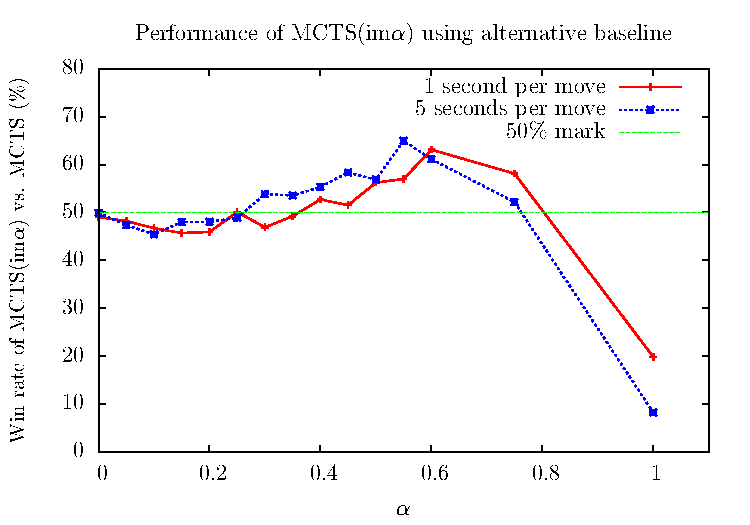
\includegraphics[scale=0.68]{plots/bt-alt-alpha}
\caption{Results of varying $\alpha$ in Breakthrough using the alternative baseline player.
Each point represents 1000 games.} 
\label{fig:bt-alt-alpha}
\end{center}
\end{figure}

%Through systematic testing, we found the best baseline with this evaluation 
%function to use the pd$20$ playout. 

\subsection{Kalah}

\begin{figure}
\begin{center}
\includegraphics[scale=0.68]{plots/kalah-alpha}
\caption{Results in Kalah. Each data point is based on roughly 1000 games; win percentages are $\pm \approx$ 3.0\% 
with 95\% confidence.}
\label{fig:loa-alpha}
\end{center}
\end{figure}

Kalah is a turn-taking game in the Mancala family of games. Each player has six houses, each 
initially containing four stones, and a store on the endpoint of the board, initially empty. 
On their turn, a player chooses one of their houses, removes all the stones in it, and ``sows'' 
the stones one per house in counter-clockwise fashion, skipping the opponent's store. 
If the final stone lands in the player's store, that player gets another turn, and there is no 
limit to then number of consecutive turns taken by same player. If the stone ends on a house owned
by the player that contains no stones, then that player captures all the stones in the adjacent 
opponent house, putting it into the player's store. The game plays until one player's houses are
all empty; the opponent then moves their remaining stones to their store. The winner is the player
who has collected the most stones in their store. 
Kalah has been weakly solved for several different variants of Kalah~\cite{Irving00Solving}, 
and was used as a domain to compare MCTS variants to classic minimax search~\cite{Ramanujan11Tradeoffs}.

In running experiments from the initial position, we observed a noticeable first-player bias. Therefore, as
was done in \cite{Ramanujan11Tradeoffs}, our experiments produce random starting board positions 
without any stones placed in the stores. 
Competing players play one game and then swap seats to play a second game using the same board. A player 
is declared a winner if that player won one of the games and at least tied the other game. If the same side 
wins both games, the game is discarded. 
Tournament results revealed that a pd$4$ early termination worked best. 
The evaluation function was simply the difference between stones in each player's stores. Results with one 
second of search time are shown in Figure~\ref{fig:loa-alpha}. 
%As with the previous study employing MCTS, we notice that an evaluation function can be used to enhance the performance.
Here, we again notice the same patterns as in Breakthrough. Within the range $\alpha \in [0.1,0.5]$ there is a clear 
advantage in performance when using implicit minimax backups against the base player. 

\subsection{Lines of Action}

\begin{figure}[t]
\begin{center}
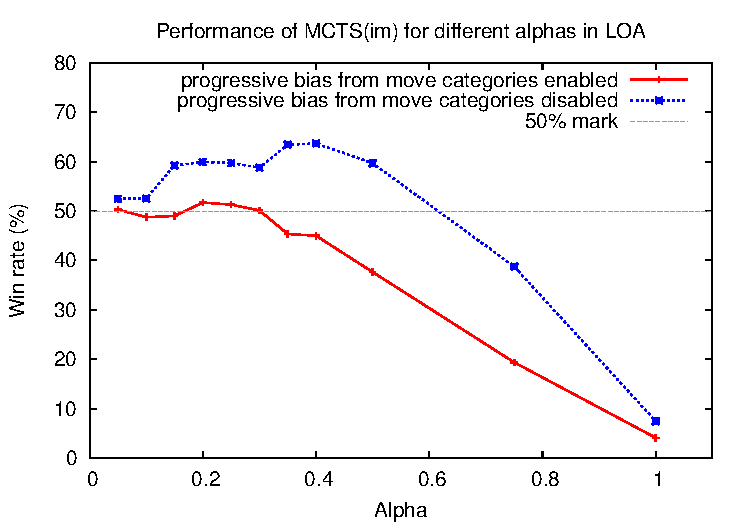
\includegraphics[scale=0.7]{plots/loa-alpha}
\caption{Results in LOA. Each data point represents 1000 games with 1 second of search time. } 
\label{fig:loa-alpha}
\end{center}
\end{figure}

\begin{table}[t]
{\small
\begin{center}
\begin{tabular}{ccccc|c}
Options & Player        & Opp. & $n$ & $t$ & Res. (\%) \\
\hline
\hline
PB      & MCTS(im$\alpha$) & MCTS     & 32000 & 1        & 50.59       \\
PB      & MCTS(im$\alpha$) & MCTS     & 6000  & 5        & 50.91       \\
\hline
$\neg$PB & MCTS(im$\alpha$) & MCTS & 1000 & 1  & 59.90       \\
$\neg$PB & MCTS(im$\alpha$) & MCTS & 6000 & 5  & 63.10       \\
$\neg$PB & MCTS(im$\alpha$) & MCTS & 2600 & 10 & 63.80       \\
\hline
$\neg$PB & MCTS             & $\alpha \beta$ & 2000 & 5  & 40.0       \\
$\neg$PB & MCTS(im$\alpha$) & $\alpha \beta$ & 2000 & 5 & 51.0       \\
\hline
PB       & MCTS             & $\alpha \beta$ & 5800 & 5  & 61.8       \\
PB       & MCTS(im$\alpha$) & $\alpha \beta$ & 5800 & 5  & 62.6       \\
\hline
\end{tabular}
\end{center}
\caption{Summary of results for players and opponent pairings in LOA. 
All MCTS players use $\alpha \beta$ playouts and MCTS(im$\alpha$) players use $\alpha = 0.2$. 
Here, $n$ represents the number of games played and $t$ time in seconds per search.}
\label{tbl:loaresults}
}
\end{table}

LOA is a turn-taking alternating-move game played on an 8-by-8 board that uses checkers board and pieces.
The goal is to connect all your pieces into a single connected group (of any size), 
where the pieces are connected via adjacent and diagonals squares. A piece may move in any direction, but the number of squares 
it may move depends on the total number of pieces in the line, including opponent pieces. A piece may jump over its own
pieces but not opponent pieces. Captures occur by landing on opponent pieces. 

For LOA, we have based our MCTS implementation and enhancements on the state-of-the-art techniques described in \cite{Winands10MCTS-LOA}, 
which has won several Computer Olympiad tournaments and is to the best of our knowledge the world's best AI for Lines of Action.
The evaluation function used is the one based on the features used in MIA~\cite{Winands06MIA}.
All of the results in LOA are based 100 opening board 
positions.\footnote{\small https://dke.maastrichtuniversity.nl/m.winands/loa/} 

We repeat the implicit minimax backups experiment with varying $\alpha$. At first, we use standard UCT without enhancements 
and a simple playout that is selects moves non-uniformly at random based on the move categories, and uses the early cut-off strategy. 
Then, we enable shallow $\alpha \beta$ searches in the playouts described in~\cite{Winands11AB}. 
Finally, we enable the progressive bias based on move categories. The results for these 
three different settings are shown in Figure~\ref{fig:loa-alpha}. As before, we notice that in the first two situations,
implicit minimax backups with $\alpha \in [0.1,0.5]$ can lead to better performance. When the progressive bias based on move 
categories is added, the advantage diminishes. However, we do notice that $\alpha \in [0.05,0.3]$ seems to not significantly 
decrease the performance. 

Additional results are summarized in Table~\ref{tbl:loaresults}. From the graph, we reran $\alpha = 0.2$ with progressive bias for 
32000 games giving a statistically significant (95\% confidence) win rate of 50.59\%. 
We also tried increasing the search time, in both cases (with and without progressive bias), 
and observed a gain in performance at five and ten seconds. 
In the past, the strongest LOA player was MIA which was based on $\alpha \beta$ search. Therefore, we also test our MCTS with 
implicit minimax backups against an $\alpha \beta$ player based on MIA. When progressive bias is disabled, implicit minimax backups
increases the performance by 11 percentage points. There is also a small (but statistically insignificant) increase in 
performance when progressive bias is enabled. 
Also, at $\alpha = 0.2$, it seems that there is no statistically significant case of implicit minimax backups hurting performance. 

\subsubsection{Discussion: Limitations.} While we have shown positive results in a number of domains, we recognize that this 
technique is not universally applicable. We believe that implicit minimax backups work because there is short-term tactical 
information which 
is not captured in the long-term playouts, but is captured by the implicit minimax procedure. Additionally, we suspect that 
there must be strategic 
information in the playouts which is not captured in the shallower minimax backups. Thus, success depends on both the domain and 
the evaluation function used. Implicit minimax backups did not improve performance in Chinese Checkers or the card game Hearts, 
but more work needs to be done to understand if we would find success with a better evaluation function.

\section{Conclusion}

We have introduced a new technique called implicit minimax backups for MCTS. 
Unlike previous methods, this techniques stores 
the information from both sources separately, only combining the two sources to guide
selection. This simple technique can lead to stronger play even with
basic evaluation functions, in Breakthrough and Kalah. Furthermore, the technique improves 
performance in LOA, a larger, more complex domain with sophisticated knowledge and 
strong MCTS and classic $\alpha \beta$ players.

For future work, we would like to apply the technique in other games, Amazons in 
particular. 
We aim to compare the technique with sufficiency thresholds 
of Gudmundsson \& Bj\"{o}rnsson (2013). 
%We also plan to investigate decaying strategies for 
%$\alpha$ and incremental $\alpha \beta$ pruning.
The technique could also work in general game-playing agents using 
evaluations learned during search~\cite{Finnsson10Learning}.

\bibliographystyle{aaai}
\bibliography{im-mcts}


\end{document}
